\documentclass[]{article}
\usepackage[UTF8]{ctex}
\usepackage{graphicx}
\usepackage{xcolor}
\usepackage{float}
\usepackage{listings}
\usepackage{makecell}
\usepackage{subfigure}
\usepackage{ulem}
\graphicspath{{./pics/}}
\usepackage[colorlinks,
            linkcolor=blue,
            urlcolor=cyan,
            citecolor=green
            ]{hyperref}
\definecolor{vgreen}{RGB}{104,180,104}
\definecolor{vblue}{RGB}{49,49,255}
\definecolor{vorange}{RGB}{255,143,102}
\lstset{
    basicstyle          =   \sffamily,          % 基本代码风格
    keywordstyle        =   \bfseries,          % 关键字风格
    commentstyle        =   \rmfamily\itshape,  % 注释的风格,斜体
    stringstyle         =   \ttfamily,  % 字符串风格
    flexiblecolumns,                % 别问为什么,加上这个
    numbers             =   left,   % 行号的位置在左边
    showspaces          =   false,  % 是否显示空格,显示了有点乱,所以不现实了
    numberstyle         =   \zihao{-5}\ttfamily,    % 行号的样式,小五号,tt等宽字体
    showstringspaces    =   false,
    captionpos          =   t,      % 这段代码的名字所呈现的位置,t指的是top上面
    breaklines      =   true,
    frame               =   lrtb,   % 显示边框
}
\lstdefinestyle{verilog-style}
{
    language=Verilog,
    basicstyle=\small\ttfamily,
    keywordstyle=\color{vblue},
    identifierstyle=\color{black},
    commentstyle=\color{vgreen},
    numbers=left,
    numberstyle=\tiny\color{black},
    numbersep=10pt,
    tabsize=8,
    breaklines      =   true,   
    moredelim=*[s][\colorIndex]{[}{]},
    literate=*{:}{:}1
}
\lstdefinestyle{python-style}
{
    language=Python,
    basicstyle=\small\ttfamily,
    keywordstyle=\color{vblue},
    identifierstyle=\color{black},
    commentstyle=\color{vgreen},
    numbers=left,
    numberstyle=\tiny\color{black},
    numbersep=10pt,
    tabsize=8,
    breaklines      =   true,   
    moredelim=*[s][\colorIndex]{[}{]},
    literate=*{:}{:}1
}
\lstdefinestyle{c-style}
{
    language=C,
    basicstyle=\small\ttfamily,
    keywordstyle=\color{vblue},
    identifierstyle=\color{black},
    commentstyle=\color{vgreen},
    numbers=left,
    numberstyle=\tiny\color{black},
    numbersep=10pt,
    tabsize=8,
    breaklines      =   true,   
    moredelim=*[s][\colorIndex]{[}{]},
    literate=*{:}{:}1
}

\makeatletter
\newcommand*\@lbracket{[}
\newcommand*\@rbracket{]}
\newcommand*\@colon{:}
\newcommand*\colorIndex{%
    \edef\@temp{\the\lst@token}%
    \ifx\@temp\@lbracket \color{black}%
    \else\ifx\@temp\@rbracket \color{black}%
    \else\ifx\@temp\@colon \color{black}%
    \else \color{vorange}%
    \fi\fi\fi
}
\makeatother

\usepackage{fancyhdr}
\pagestyle{fancy}

\usepackage{trace}
\begin{document}
  \begin{titlepage}
    \centering


    \rule{\textwidth}{1pt}   % The top horizontal rule
    
    \vspace{0.03\textheight}

    {\LARGE 数字逻辑电路与计算机组成实验}
    
    \vspace{0.015\textheight}
    {\Huge RISCV五段流水线CPU设计}

    \vspace{0.03\textheight}   

    \rule{0.83\textwidth}{0.4pt} 

    \vspace{0.1\textheight} 


    \begin{center}
            \Large 姓名:\ \ \underline{\makebox[200pt]{******}}\\
            \vspace{0.02\textheight}
            \Large 学号:\ \ \underline{\makebox[200pt]{******}}\\
            \vspace{0.02\textheight}
            \Large 邮箱:\ \ \underline{\makebox[200pt]{201220013@smail.nju.edu.cn}}
    \end{center}

    \vfill 

    {\large \today}
    \vspace{0.1\textheight} 


    \rule{\textwidth}{1pt} 

  \end{titlepage}
  
  
  \tableofcontents
  
  \newpage
  \section{项目概览}
  \subsection{硬件部分}
  \begin{enumerate}
      \item \textbf{RISC-V五段流水线CPU}:实现了\textit{取指-译码-执行-访存-回写}的流水线CPU,包含转发与阻塞探查处理,常见数据冒险无冲刷,load-use指令插入一次气泡。
      \item \textbf{中断与CSR寄存器支持}:实现了流水线的中断,支持机器态、非向量、无嵌套的中断处理。添加CSR寄存器及CSR读写指令(csrrc、csrrw等6条),添加ecall、mret指令。实现时钟中断。
      \item \textbf{板载硬件支持与显示器拓展}:支持内核写入板上6个七段数码管与10个LEDR,支持VGA字符的最高256色显示
      \item \textbf{内存映射与IO调度}:利用内存映射实现代码区、数据区、显存、键盘数据、中断临时栈等无冲突读写
  \end{enumerate}
  \subsection{软件部分}
  \begin{enumerate}
      \item \textbf{内核编写}:使用C语言编写内核,提供了输入输出接口、常见std函数(strtok、atoi、strcmp、itoa)、软件乘除法,兼具易用性与可拓展性。实现几条要求的基础指令。
      \item \textbf{中断注册与处理}:使用汇编语言编写中断处理入口函数、完成状态保存与上下文切换,C语言使用内联汇编方式编写中断注册与实际处理函数,实现了时钟中断处理。
      \item \textbf{移植表达式求值、实现跑马灯功能}:移植了PA的表达式求值,可以实现常见的表达式求值。利用板载硬件的内存映射完成类似开发板开机时的跑马灯功能。
      \item \textbf{字符动画}:基于之前写的字符动画脚本实现了字符动画。利用字符串压缩算法大幅减小存储占用,压缩率9\%,使用128KB内存可以播放约30s。
  \end{enumerate}
  \subsection{其他}
  \begin{enumerate}
      \item \textbf{编写调试辅助脚本}:编写了一个python脚本,可以交互式地将16进制Riscv指令转换为汇编,方便调试
  \end{enumerate}
  
  
  \section{硬件部分}
  \subsection{基础五段流水线}
  首先贴上一张《计算机系统基础》课程的ppt内容,下图展示了一个基本的五段流水线CPU的工作流程,也即\textit{取指-译码-执行-访存-回写}五个步骤,理想状态下流水想上始终有5个指令在并行执行。
  \begin{figure}[htb]
      \centering
      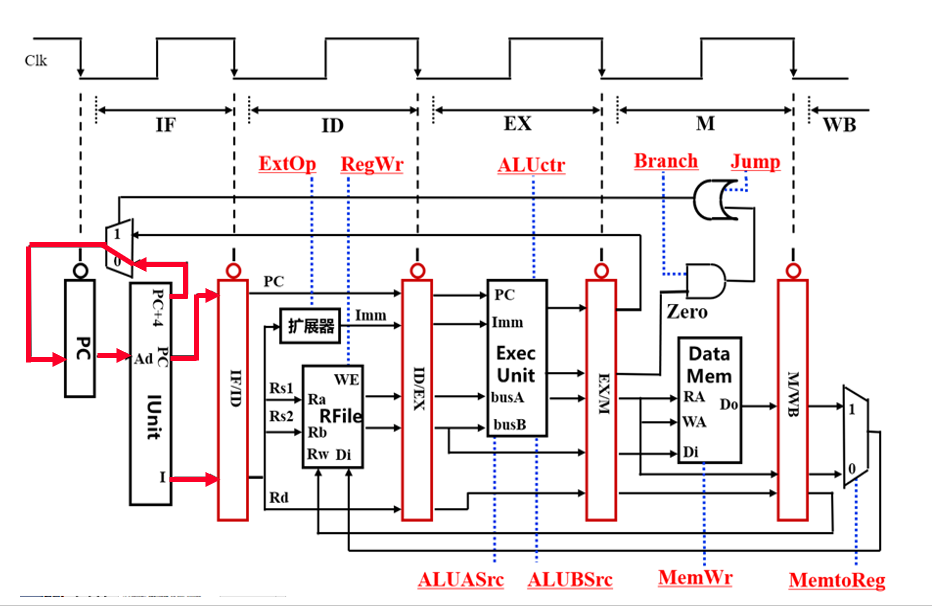
\includegraphics[width=0.8\textwidth]{pipeline.png}
      \caption{5段流水线原理图}
      \label{fig:pipeline}
  \end{figure}
  
  本项目的流水线基本遵循了这一结构,只是在branch部分稍作修改,以符合实验十一的指令译码,在后续的中断支持部分添加了一些特有的部件,不过不影响当前这一部分的执行。
  
  可以看到,流水线的设计分为10个主要部分,5个流水线寄存器、5个执行部件,我们的主要工作就是完成分别完成他们,做好他们之间的连线。这一部分在\textbf{hardware/cpu/pipelilne.v}中。
  
  在具体阐述每个部件的工作之前,我们先明确一下整个项目的时序设计,整体上时序遵循存储器与通用寄存器堆上升沿读写、内部数据下降沿写入上升沿使用的逻辑,具体分配如下:
  \begin{enumerate}
      \item \textbf{上升沿}:流水线控制器、中断控制器、通用寄存器与CSR寄存器写入、RAM读写
      \item \textbf{下降沿}:流水段寄存器、PC、中断信号发生器
  \end{enumerate}
  其他例如时钟中断发生器、VGA控制器、PS2控制器的时钟沿实际上并不那么严格。
  \subsubsection{流水线控制信号}
  流水线的行为是比较复杂的,正常情况下5个状态依此向前流动,也有不少特殊情况,如当branch跳转来临时,需要冲刷MEM之前的所有寄存器,如中断信号来临时,应该暂停流水线以便做好状态保存,保存之后又要冲刷掉所有流水段寄存器内容进入中断处理。因而项目设置了一个\textit{pipeline\_status}模块,根据若干控制信号生成5个流水段寄存器以及PC的控制信号,信号宽度3bit,以define的形式写在\textbf{hardware/cpu/define.v}中。外界信号的响应有\textbf{优先级},从高到低分别为:全局reset信号、中断信号、中断预处理的流水线暂停、跳转、load-use阻塞、正常工作。
  
  \begin{lstlisting}[style={verilog-style}]
  module pipeline_status (
   input clr,
   input clk,
   input branch,
   input stall,
   input int_set_pl_pause,
   input int_flag,

   input [31:0] int_pc,

   output [`PL_STATUS_BUS_WIDTH] pl_ctrl_pc_out,
   output [`PL_STATUS_BUS_WIDTH] pl_ctrl_ID_out,
   output [`PL_STATUS_BUS_WIDTH] pl_ctrl_EX_out,
   output [`PL_STATUS_BUS_WIDTH] pl_ctrl_MEM_out,
   output [`PL_STATUS_BUS_WIDTH] pl_ctrl_WB_out,

   output reg [31:0] int_pc_out
  );
  //具体信号生成见代码
  endmodule
  \end{lstlisting}
  \subsubsection{取指模块IF}
  IF段包含了PC以及指令的获取,流水线的模块中并不包括Instruction RAM,IF段会引出地址引脚、引入读取到的地址,提供的引脚如下:
  \begin{lstlisting}[style={verilog-style}]
  module IF (
    input               clr,
    input               clk,
    
    input       [31:0]  pc,
    output      [31:0]  instr,

    input       [31:0]  imemdataout,
    output      [31:0]  imemaddr,
    output              imemclk
  );

  \end{lstlisting}
  
  PC被分离为一个单独的模块,根据控制信号选择不同的nextpc:
  \begin{lstlisting}[style={verilog-style}]
  always @(negedge clk) begin
   if(PL_status == `PL_FLUSH) 
      pc <= 0;
   else if(PL_status == `PL_PC_INT)
      pc <= nextpc_int;
   else if(PL_status == `PL_PC_BRANCH)
      pc <= nextpc_mem;
   else if(PL_status == `PL_PAUSE)
      pc <= pc;
   else if(PL_status == `PL_NORMAL)
      pc <= pc + 4;
   else
      pc <= 0;
  end
  \end{lstlisting}
  \subsubsection{译码模块ID}
  IF与ID之间有一个IF\_ID\_reg模块,存储流水信息,在这里只存储了指令与PC,下面的4个流水段寄存器中还会存储控制信号在内的很多信息,不过大同小异,在这里给下整体框架,后续将不再赘述各个流水段寄存器的行为了。
  \begin{lstlisting}[style={verilog-style}]
    module IF_ID_reg (
        input       [`PL_STATUS_BUS_WIDTH]   pl_ctrl_ID,
        input               clk,
        input       [31:0]  pc_in,
        input       [31:0]  instr_in,
        output  reg [31:0]  pc_out,
        output  reg [31:0]  instr_out
    );
    
    always @(negedge clk) begin
        if(pl_ctrl_ID == `PL_FLUSH) begin
            pc_out <= 32'd0;
            instr_out <= 32'd0;
        end else if(pl_ctrl_ID == `PL_PAUSE) begin
            pc_out <= pc_out;
            instr_out <= instr_out;
        end else begin
            pc_out <= pc_in;
            instr_out <= instr_in;
        end
    end
  \end{lstlisting}
  
  ID模块的主要工作是根据取到的Instruction进行指令译码,生成控制信号\textit{extop, regwr, ALUAsrc, ALUBsrc, ALUctr, branch, MemtoReg, memwr, memop}(这一部分不会提及有关中断的控制信号与各个引脚)并生成立即数。控制信号生成器直接使用实验十一的\textbf{control\_gen}模块,这里不再详述,ID模块主体代码如下:
  \begin{lstlisting}[style={verilog-style}]
    module ID (
    //若干引脚
    );
    
    assign rd = instr[11:7];
    assign rs1_addr = instr[19:15];
    assign rs2_addr = instr[24:20];
    contr_gen contr_gen_instance(...);
    imm_gen imm_gen_instance(instr, extop, imm);
    
    assign csr_raddr = {20'd0, imm[11:0]};  //这两行是中断支持
    assign csr_data_out = csr_rdata;
        
    endmodule
  \end{lstlisting}
  \subsubsection{执行模块EX}
  执行模块使用ID\_EX\_reg流水段寄存器输出的内容,传入ALU中进行运算并输出aluresult,算术运算部分也是完全沿用了实验十一的相关内容,只不过两个输入需要考虑转发(处理后为rs1\_proc, rs2\_proc),EX模块中还会并行计算出可能的两个跳转地址传入下一个流水段寄存器.主体代码如下:
  \begin{lstlisting}[style={verilog-style}]
    module EX (
        //若干引脚
    );
    
    wire [31:0] dataa;
    wire [31:0] datab;
    
    wire [31:0] rs1_proc = forward_rs1[0] ? aluresult_wb : (forward_rs1[1] ? aluresult_mem : rs1);
    wire [31:0] rs2_proc = forward_rs2[0] ? aluresult_wb : (forward_rs2[1] ? aluresult_mem : rs2);
    
    assign rs2_forward = rs2_proc;
    assign nextpc_pc = pc + imm;
    assign nextpc_rs1 = rs1_proc + imm;
    assign dataa = ALUAsrc?pc:rs1_proc;
    assign datab = (ALUBsrc==2'b00 ? rs2_proc : (ALUBsrc==2'b01 ? imm : 32'd4));
    alu alu_instance(dataa, datab, ALUctr, less, zero, aluresult);
    CSRALU csr_alu_instance(csr_data, rs1_proc, {27'd0, zimm}, csr_aluctr, csr_aluresult); //CSR指令专用ALU
        
    endmodule
  \end{lstlisting}  
  \subsubsection{访存模块MEM}
  访存模块也没有实例化RAM,只是做了一个引脚的连接来调用外界的RAM,再将输出送给下一个流水段寄存器。在MEM模块中还做了跳转的判断,这样可以最大限度地减少跳转带来的流水线冲刷,如果需要跳转,在MEM模块就会将branch信号送出,并给出nextpc的值。
  \begin{lstlisting}[style={verilog-style}]
    module M (
        //若干引脚
    );
    
    assign dmemaddr = aluresult;
    assign dmemdatain = rs2;
    assign dmemrdclk = clk;
    assign dmemwrclk = clk;
    assign dmemop = memop;
    assign dmemwe = memwr;
    
    assign dmemdata = dmemdataout;
    
    wire PCAsrc, PCBsrc;
    branch_cond branch_cond_instance(less, zero, branch, PCAsrc, PCBsrc);
    assign nextpc = PCBsrc?nextpc_rs1:nextpc_pc;
    assign pc_branch = PCAsrc?1'b1:1'b0;
    endmodule
  \end{lstlisting}    
  \subsubsection{回写模块WB}

  回写模块事实上并没有作什么工作,只是根据memtoreg和下面的csr2reg选择合适的busW传入通用寄存器堆,通用寄存器堆会根据regwr选择进行写入操作。

  \begin{lstlisting}[style={verilog-style}]
    module WB (
        //若干引脚
    );
    assign busW = csr2reg ? csr_aluresult : (MemtoReg?dmemdata:aluresult);
    endmodule
  \end{lstlisting}    
  \subsection{冒险与Load-Use阻塞}
  流水线的5段处理大大增加硬件使用效率的同时也带来了诸多问题,流水线有三种常见冒险:
  \begin{itemize}
      \item 结构冒险:如果一条指令需要的硬件部件还在为之前的指令工作,而无法为这条指令提供服务,那就导致了结构冒险。
      \item 数据冒险:如果一条指令需要某数据而该数据正在被之前的指令操作,那这条指令就无法执行,就导致了数据冒险
      \item 控制冒险:如果现在要执行哪条指令,是由之前指令的运行结果决定,而现在那条之前指令的结果还没产生,就导致了控制冒险。
  \end{itemize}
  
  \textbf{结构冒险}方面,指令寄存器与数据寄存器已经被分开,通用寄存器设置为上升沿写入、下降沿有效,规避了两种结构冒险。
  
  \begin{figure}[htb]
      \centering
      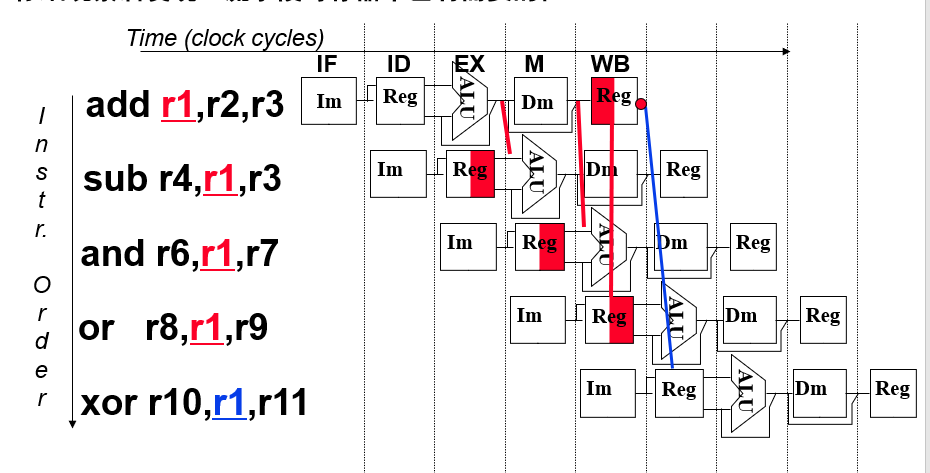
\includegraphics[width=0.8\textwidth]{forward.png}
      \caption{3种需要转发的流水线状态}
      \label{fig:forward}
  \end{figure}
  \textbf{数据冒险}方面,当一条指令的运算结果需要写入某个寄存器,且这个寄存器的值需要被下两条中的某个取用时会发生数据冒险,因为此时正确的运算结果还没有写入寄存器,ID阶段取出的值还是不正确的。处理这种冒险的方式有很多种,这里采用\textbf{转发}的方式解决。观察发现,冒险发生时,正确的结果已经被计算出来,虽然从regfile中取到的值是不正确的,我们可以从EX-M或者M-WB流水段寄存器中转发正确的结果,只需要一个模块进行判断是否需要转发即可。在forward\_detecter模块中,根据EX阶段的两个寄存器地址值与M、WB两阶段写回的地址与使能信号,判断是否需要转发,输出转发控制信号,优先级方面,WB转发优先于M转发,代码如下:
  \begin{lstlisting}[style={verilog-style}]
    module forward_detecter(
       input                regwr_mem,
       input                regwr_wb,
       input      [4 : 0]   rs1,
       input      [4 : 0]   rs2,
       input      [4 : 0]   rd_addr_mem,
       input      [4 : 0]   rd_addr_wb,
       // forward ctrl: 00 = no forward, 01 = forward from m/wb, 10 = forward from ex/mem
       output 	  [1 : 0]   forward_rs1,
       output     [1 : 0]   forward_rs2
      );
    
    // forward rs1, mem first
    wire tmp_rs1 = regwr_mem && (rs1 == rd_addr_mem);
    assign forward_rs1[1] = rs1 != 5'h0 && tmp_rs1;
    assign forward_rs1[0] = rs1 != 5'h0 && regwr_wb && !tmp_rs1 && (rs1 == rd_addr_wb);
    
    // forward rs2
    wire tmp_rs2 = regwr_mem && (rs2 == rd_addr_mem);
    assign forward_rs2[1] = rs2 != 5'h0 && tmp_rs2;
    assign forward_rs2[0] = rs2 != 5'h0 && regwr_wb && !tmp_rs2 && (rs2 == rd_addr_wb);
    
    endmodule
  \end{lstlisting}  

  
  还剩下一种数据冒险没有解决:\textbf{load-use冒险},寄存器写入在第四周期,而回写在下一周期,如果load的下一条指令需要访存出来的值,我们无妨通过转发的方式将正确的值送过去,这里我们采用的解决方案是在检测到load-use情况时加入一条“气泡”,ID阶段刚结束的指令不进入EX阶段,而是暂停一周期,等待WB执行完得到正确的值。具体到代码上,就是ID\_EX\_reg的控制信号设为flush,PC与IF\_ID\_reg的控制信号设为PAUSE,后面的为NORMAL。load-use的判定为:位于EX阶段的指令mem2reg为真,且写入地址与下一条指令的某一个寄存器地址相同。
  \begin{lstlisting} [style={verilog-style}]
  module load_use_detecter (
   input            mem2reg_ex,
   input  [4 : 0]   rd_addr_ex,
   input  [4 : 0]   rs1_addr_id,
   input  [4 : 0]   rs2_addr_id,
   output           stall
    );
    assign stall = mem2reg_ex && ((rd_addr_ex == rs1_addr_id) || (rd_addr_ex == rs2_addr_id));
    endmodule
  \end{lstlisting}
  \begin{figure}[htb]
      \centering
      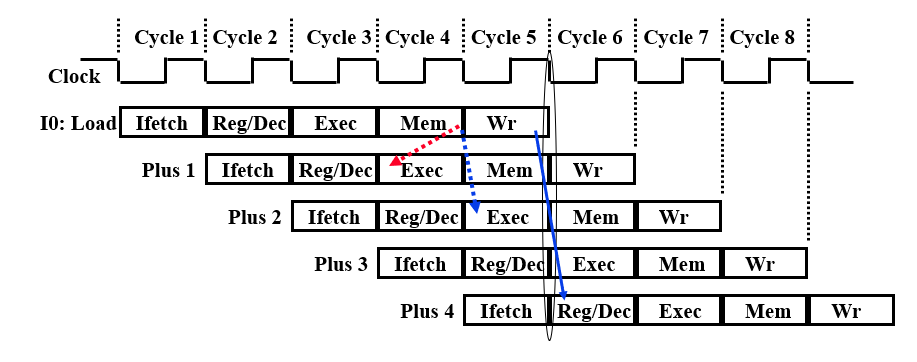
\includegraphics[width=0.8\textwidth]{load-use.png}
      \caption{load-use冒险的流水线状态}
      \label{fig:load-use}
  \end{figure}
  \subsection{基础流水线调试与DEBUG}
  至此,五段流水线的基本功能理论上实现完毕,不过整体逻辑、连线复杂,很容易出现各种bug。DEBUG方面,项目对实验十一提供的cpu-batch稍加修改即可适用于流水线。主要修改了run这个task,原本testbanch会在检测到$idataout==32'hdead10cc$时退出,而流水线下有可能这条指令被branch冲刷掉,并没有执行完,因而需要继续执行四个周期,确认这四个周期都没有发生branch。其他代码几乎不用改变,只需要把取到寄存器的链式引用改下,run部分代码修改如下:
  \begin{lstlisting} [style={verilog-style}]
    task run;
       integer i;
       integer cont;
    	begin
    	   	i = 0;
    		cont = 1;
    	   	while(cont != 0) begin
    		   	cont = 0;
    			while( (idataout!=32'hdead10cc) && (i<maxcycles))
    			begin
    				step();
    				i=i+1;
    			end
    			if(mycpu.pc_branch!=0) begin cont = 1; step(); end
    			else begin
    				if(cont != 1) begin step(); if(mycpu.pc_branch!=0) cont = 1; end
    				if(cont != 1) begin step(); if(mycpu.pc_branch!=0) cont = 1; end
    				if(cont != 1) begin step(); if(mycpu.pc_branch!=0) cont = 1; end
    				if(cont != 1) begin step(); if(mycpu.pc_branch!=0) cont = 1; end
    			end
    		end
    	end
    endtask
  \end{lstlisting}  
  大多数bug还是出在转发与连线这两方面。
  
  实验中,由于实验十一提供的hex代码是修改过的,通过官方riscv-test反汇编并不能得到,常常需要知道某串十六进制执行究竟是什么,因而编写了一个简单的Python脚本,其原理如下:首先编写一个只有一条指令的汇编文件,用gcc编译出.o文件,脚本定位到这个指令的偏移位置,用输入的十六进制串替换它,再送给objdump截取汇编代码(通过subprocess实现)。脚本主要函数代码如下:
  \begin{lstlisting}[style=python-style]
offset = 0x34
obj_src = bytearray(b"编译出的.o文件的二进制")

def decode(instr_str):
    obj = obj_src
    instr = bytearray(bytes.fromhex(instr_str))
    instr = instr[::-1] #小端
    obj[offset:offset+len(instr)] = instr
    obj = bytes(obj)
    output = open("tmp.o", "wb")
    output.write(obj)
    output.close()
    p = subprocess.Popen(["./riscv32-unknown-linux-gnu-objdump", '-d', 'tmp.o'], stdout = subprocess.PIPE)
    msg = p.stdout.read()
    msg = msg.splitlines()[-1].decode('utf-8')
    os.remove("tmp.o")
    return msg
  \end{lstlisting}
  \subsection{中断、CSR寄存器与M拓展指令}
  \subsubsection{流水线中断控制器client}
  riscv与x86的中断在核心思想上比较相近,不过具体实现上还是有颇多不同的。x86的基地址存储在idt中,而RISC下有一个专用的CSR寄存器MTVEC用于存储基地址,根据官方手册第十章,RISCV一共有8个控制状态寄存器(CSR),这里我们舍弃几个用不到的,保留mtvec, mepc, mcause, mscratch, mstatus五个,同时简化mstatus中的内容,由于我们处理非向量中断,且不嵌套,因而只保留其mie位(全局中断使能,第4位),同时也舍弃了mie寄存器。在标准中CSR寄存器地址20位有各种用途,这里全部设置为0。
  
  标准中断处理的流程如下(经过简化):
  \begin{enumerate}
      \item 异常指令的 PC被保存在 mepc中,PC被设置为mtvec。(对于同步异常,mepc指向导致异常的指令;对于中断,它指向中断处理后应该恢复执行的位置。)
      \item 根据异常来源设置 mcause,(并将 mtval设置为出错的地址或者其它适用于特定异常的信息字。舍弃)
      \item 把控制状态寄存器mstatus中的MIE位置零以禁用中断(并把先前的 MIE值保留到 MPIE中,这一过程舍弃)
      \item (不做权限处理)
  \end{enumerate}
  
  本项目中中断处理流程如下:
  \begin{enumerate}
      \item 中断控制器(client)检测到硬中断引脚有一个1且中断使能为1时进入中断预处理,暂停流水线、改变int\_state状态机。
      \item 根据int\_state用状态机在几个时钟内完成相应的csr寄存器写入操作。软硬中断下保存pc(如果正好在跳转,就保存处理后的跳转地址)到mepc,然后依此保存mstatus、mcause。mret状态下,恢复mstatus。
      \item 将int\_flag置1,并给出int\_addr,流水线控制器探查到int\_flag后进入中断相应状态,冲刷流水线,设置新的pc,进入中断处理。
  \end{enumerate}
  
  在\textbf{hardware/cpu/client.v}中,可以看到四个always语句。(代码较长这里就不贴了)
  \begin{enumerate}
      \item 第一个用组合逻辑控制int\_state状态机
      \item 第二个是csr\_state的状态转移,默认在CSR\_STATE\_IDLE空状态,检测到int\_state改变,保存当前pc、mcause并进入处理,有两种状态转移:
      \begin{enumerate}
        \item 软硬中断:\textit{CSR\_STATE\_IDLE -> CSR\_STATE\_MEPC -> CSR\_STATE\_MSTATUS -> CSR\_STATE\_MCAUSE -> CSR\_STATE\_IDLE}
        \item mret:\textit{CSR\_STATE\_IDLE -> CSR\_STATE\_MRET -> CSR\_STATE\_IDLE}
      \end{enumerate}
      \item 第三个根据csr\_state进行csr寄存器的写入,因为一个周期只能写入一个寄存器,所以要通过这种方式实现,CSR\_STATE\_MEPC状态下写mpec以此类推。
      \item 第四个会在状态保存的最后一阶段发挥作用(即CSR\_STATE\_MCAUSE或者CSR\_STATE\_MRET)将int\_flag置1,抛出应该跳转的pc值。
  \end{enumerate}
  
  全局中断使能即mstatus寄存器的第三位。int\_flag会送给pipeline\_status模块,生成相应的控制信号。
  
  CSR寄存器模块按照标准定义了几个控制寄存器,同时接收来自pipeline与client的读写命令,模块支持同时读操作(不过client并没有读操作),支持cpu和client同时写不同的寄存器,当二者写同一个寄存器时,会按照一定优先级,不过本项目中不应该出现这种情况。
  \subsubsection{CSR寄存器读写指令与mret指令}
    \begin{figure}[htb]
      \centering
      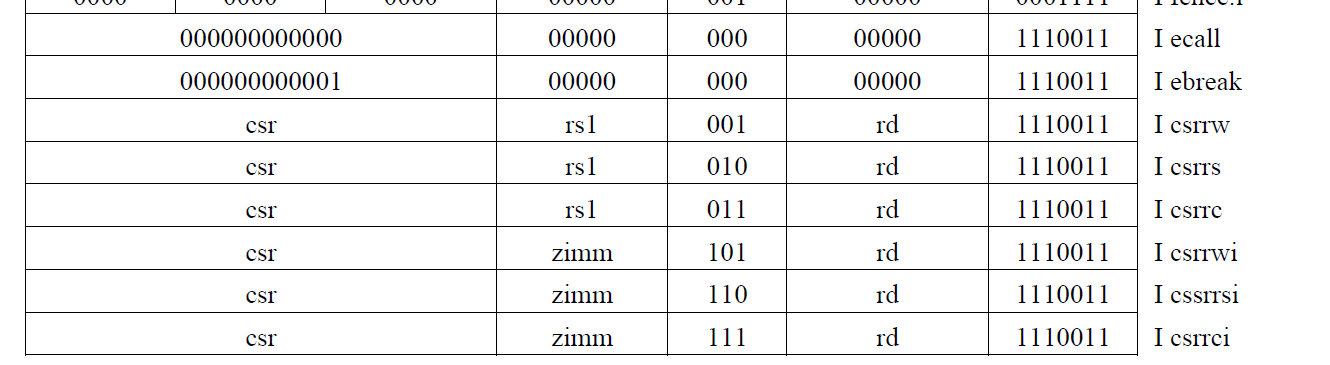
\includegraphics[width=\textwidth]{csr-instrs.png}
      \caption{添加的几条指令}
      \label{fig:csr-instrs}
  \end{figure}  
  在操作系统(Kernel下同)启动时,需要作中断注册,写入mtvec等CSR寄存器,因而还要支持CSR寄存器写入指令。项目实现了ecall指令,不过没有将输入输出处理成ecall的方式。
  
  观察其指令形式,对比现有的指令执行过程,可以发现csr部分就是I型立即数,rs1和rd正常解码,唯一有区别的就是EX模块和WB模块,EX模块为了不改变原来的ALU,项目中添加了专用的CSR\_ALU与csr\_aluctr,WB模块添加了csr2reg,csr\_we两个控制信号。
  
  根据手册,可以看出CSR\_ALU需要三个输入:rs1,zimm,csr,输出的值被写入到某个通用寄存器中。下面是拓展后的控制信号(未提到的都为0):
  \begin{table}[h!]
      \centering
      \begin{tabular}{c|c|c|c|c|c|c|c}
         \hline
           指令 & op[6:2] & func3 & ExtOp & RegWr & csralu\_ctr & csr2reg & csr\_we  \\
         \hline
        csrrw & 11100 & 001 & 000 & 1 & 000 & 1 & 1 \\
        csrrs & 11100 & 010 & 000 & 1 & 010 & 1 & 1 \\
        csrrc & 11100 & 011 & 000 & 1 & 100 & 1 & 1 \\
        csrrwi & 11100 & 101 & 000 & 1 & 001 & 1 & 1 \\
        cssrrsi & 11100 & 110 & 000 & 1 & 011 & 1 & 1 \\
        csrrci & 11100 & 111 & 000 & 1 & 101 & 1 & 1 \\
        ecall & 11100 & 000 & 000 & 0 & 000 & 1 & 0  \\
        \hline
      \end{tabular}
      \caption{拓展指令译码表}
      \label{tab:csrinstrs}
  \end{table}
  
  \begin{table}[h!]
      \centering
      \begin{tabular}{c|c}
        \hline
        csraluctr & operation \\
        \hline
        000 & rs1 \\
        001 & zimm \\
        010 & rs1|csr \\
        011 & zimm|csr \\
        100 & \~rs1|csr \\
        101 & \~zimm|csr \\
        \hline
      \end{tabular}
      \caption{CSR\_ALU控制信号}
      \label{tab:csraluctr}
  \end{table}
  
  在EX模块中添加CSR\_ALU:
    \begin{lstlisting} [style={verilog-style}]
  CSRALU csr_alu_instance(csr_data, rs1_proc, {27'd0, zimm}, csr_aluctr, csr_aluresult);
  \end{lstlisting}
  在WB模块添加csraluresult的选择:
      \begin{lstlisting} [style={verilog-style}]
  assign busW = csr2reg ? csr_aluresult : (MemtoReg?dmemdata:aluresult);
  \end{lstlisting}
  流水线模块添加csrs和client,按需修改几个流水段寄存器,完成中断的硬件支持。
  \subsubsection{时钟中断}
  项目中实现了一个时钟硬件,每1毫秒发出一次时钟中断。以时钟中断为例阐述整个中断流程:
  \begin{enumerate}
      \item Kernel启动并完成中断注册,将全局中断使能置1
      \item 时钟满足触发条件(这里为计数器小于等于7)且全局中断使能为1,将中断引脚置为1
      \item client检测到中断引脚,将全局中断使能置0。保存几个CSR寄存器,然后将int\_flag置1.
      \item 流水想控制器检测到int\_flag,冲刷流水线进入中断处理入口程序。
      \item 中断处理入口程序取出mscrach的值(临时栈地址),保存若干通用寄存器到临时栈。将mcause作为函数参数调用中断处理程序。
      \item 中断处理程序内执行处理流程。本项目中时钟中断时累加时间,并更新键盘输入。
      \item 中断处理程序返回到中断入口程序,恢复通用寄存器,执行mret指令。
      \item client检测到mret,进入mret执行,恢复mstatus等寄存器,将int\_flag置1,跳转回之前的pc。
  \end{enumerate}
  \subsection{内存映射}
  硬件IO通过内存映射的方式进行,例如VGA将固定位置的内存作为显存,读取其中的ascii码进行显示。本项目中键盘没有采用复杂的处理,键盘会始终将按下的按键同步到内存中,支持字符与ctrl、shift同时按下,但不支持多个字符一起按下。内存映射模块在\textbf{hardware/memory/memory\_map.v}中。内存分配如下:
  \begin{table}[h!]
      \centering
      \begin{tabular}{c|c|c|c}
            \hline
           起始地址 & 描述 & 读取模块 & 写入模块 \\
           \hline
           0x00000000 & 指令ROM & cpu & none\\
           0x00100000 & 数据RAM & cpu & cpu\\
           0x00200000 & VGA控制信号,包含光标位置、滚屏行数 & vga & cpu \\
           0x00300000 & VGA字符ASCII码RAM & vga & cpu \\
           0x00400000 & VGA字符颜色RAM & vga & cpu \\
           0x00500000 & \makecell{键盘信息,包含按下的按键ascii码,\\与ctrl、shift是否按下等} & cpu & keyboard \\
           0x00700000 & 临时栈,在中断时使用 & cpu & cpu \\
           0x00800000 & 数码管与LEDR & hardware & cpu \\
           0x00900000 & 字符动画内容ROM & cpu & none \\
           \hline
      \end{tabular}
      \caption{内存映射的分配}
      \label{tab:my_label}
  \end{table}
  
  内存映射模块中,实例化所有存储器,根据地址的前缀将某一个存储器的写使能置一,读写口是分开的,cpu、数码管LEDR、vga的读取互相不冲突。内存映射模块有四个方向的读写需求:来自cpu、vga、键盘和数码管LEDR,因而有若干个各自的引脚。存储器方面较大的存储器(指令ROM和数据RAM)采用IP核并且有专门的处理模块,支持memop(与实验十一相同),键盘、VGA控制信号等有实时读取需求,采用reg方式实现。
  \section{软件部分}
  硬件部分我们实现了底层,还需要操作系统来实现交互,这一部分就是完成操作系统内核的设计。这里我们采用C语言(以及少部分汇编与内联汇编)编写内核Kernel,然后RISCV32编译环境进行编译得到mif文件。
  
  在这个简易操作系统中,没有进程的概念,所有指令的执行都在内核态完成,虽然实现了ecall,不过输入输出依然是直接调用函数而非通过ecall进行陷阱操作。
  \subsection{系统API函数}
  \subsubsection{输出}
  输出。部分,为了方便缓冲的实现,输出采用64*30的大小,算上缓冲区一共64*64个字符,方便用位移快速运算。正如前面所说,有一块专门的显存用于存储ascii码,cpu只负责写,vga只负责读,在\textbf{include/global.h}中,定义了很多常量,包括各个内存区的地址前缀,显存分为两块,一个字符、一个颜色,在syscall.c中定义显存数组指针:
  \begin{lstlisting}[style={c-style}]
  uint8_t *const ch_mem = (uint8_t *)VGA_CHAR_OFFSET;
  uint8_t *const color_mem = (uint8_t *)VGA_COLOR_OFFSET;  
  \end{lstlisting}
  写显存时,只需要进行普通数组操作即可。
  
  输出时,有三个控制输出状态的变量:monitor\_write\_cursor记录当前写入点在64*64的显存中的位置,output\_front\_cursor记录退格能够退到的最前位置(例如不能删去命令提示符\$),VGAINFO类型的结构体vga\_info,用于记录光标位置、滚屏的行数,通过*p\_vga\_info = vga\_info;的方式写入。
  
  最底层输出函数\_setc,向addr写入color颜色的c:
  \begin{lstlisting}[style={c-style}]
  inline static void _setc(const char c, const uint8_t color, const uint32_t addr)
    {
        ch_mem[addr] = c;
        color_mem[addr] = color;
    }
  \end{lstlisting}
  第一层封装putc,对换行、退格、tab做了特殊处理,并且在输出之后会判断是否需要滚动屏幕:
  \begin{lstlisting}[style={c-style}]
void putc(const char c, const uint8_t color)
{
    if (c == '\n')
    {
        monitor_write_cursor = (monitor_write_cursor / COL_CNT) * (COL_CNT) + COL_CNT;
        if (monitor_write_cursor == TOTAL_CHAR + vga_info.extra_line_cnt * COL_CNT)
            scroll_screen();
        if (monitor_write_cursor == TOTAL_CHAR_WITH_BUF)
            monitor_write_cursor = 0;
    }
    else if (c == '\t')
        print("    ", COLOR_WHITE);
    else if (c == '\b')
    {
        if (output_front_cursor < monitor_write_cursor)
            _erasec(--monitor_write_cursor);
    }
    else
    {
        _setc(c, color, monitor_write_cursor++);
        if (monitor_write_cursor == TOTAL_CHAR)
            scroll_screen();
        if (monitor_write_cursor == TOTAL_CHAR_WITH_BUF)
            monitor_write_cursor = 0;
    }
    _update_cursor();
}
  \end{lstlisting}
  再一层封装print,输出color颜色的字符串str,以及辅助函数error。
  \begin{lstlisting}[style={c-style}]
  void print(const char *str, const uint8_t color)
{
    char c = *str;
    while (c)
    {
        putc(c, color);
        ++str;
        c = *str;
    }
}

inline void error(const char *msg)
{
    print("Error: ", COLOR_RED);
    print(msg, COLOR_WHITE);
}
  \end{lstlisting}
  lock\_output\_front函数用于锁定当前位置为最前位置,不允许在此位置继续退格。
  \begin{lstlisting}[style={c-style}]
inline void lock_output_front() { output_front_cursor = monitor_write_cursor; }
  \end{lstlisting}  
  \subsubsection{输入}
  由于项目采用中断的方式处理键盘输入,因而Kernel无需循环访问键盘状态,我们在kernel中维护了一个KBInfo结构,它会在时钟中断中被更新,kb\_info被声明为volatile,以便告诉编译器它随时会被修改:
  \begin{lstlisting} [style={c-style}]
  typedef struct KBInfoStruct
{
    uint8_t c;
    union 
    {
        struct
        {
            uint8_t is_shift : 1;
            uint8_t is_ctrl : 1;
            uint8_t is_caps : 1;
            uint8_t is_special : 1;
            uint8_t is_error : 1;
            uint8_t unused : 3;
        };
        uint8_t flags;
    };
} KBInfo;
exten volatile KBInfo kb_info;
  \end{lstlisting}
  
  为了判断当前kb\_info中的字符是否已经被取用过了,还需要一个InputController,记录上一个读取的字符以及读取时间:
  \begin{lstlisting} [style={c-style}]
  typedef struct InputControllerStruct
{
    uint8_t pre_c;
    uint32_t input_time;
} InputController;
  \end{lstlisting}
  一个字符被getc读取时,input\_controller被更新,另外时钟中断时如果字符发生了变化,也会更新它,这样就可以实现getc函数执行时按键按下立刻响应,同一按键保持按压时每隔\textit{KEY\_REPEAT\_INTERVAL}响应一次:
  \begin{lstlisting} [style={c-style}]
static inline bool _next_key_arrived()
{
    if (kb_info.c)
    {
        if (kb_info.c == input_controller.pre_c)
            return sys_time - input_controller.input_time > KEY_REPEAT_INTERVAL;
        else
            return kb_info.c != '\0';
    }
    else
        return false;
}
  \end{lstlisting}  
  有了next\_key\_arrived函数的帮助,getc函数也就很好写了,getc的同时还要回显,即调用putc
    \begin{lstlisting} [style={c-style}]
char getc()
{
    while (!_next_key_arrived())
        ; //wait input
    char c = kb_info.c;
    input_controller.pre_c = c;
    input_controller.input_time = sys_time;
    putc(c, COLOR_WHITE);
    return c;
}
  \end{lstlisting}
  向上封装一层getline,将一行的输入计入buf,需要注意退格的处理:
  \begin{lstlisting} [style={c-style}]
  void getline(char *buf)
{
    char c;
    int i = 0;
    while ((c = getc()) != '\n')
    {
        if (c == '\b')
        {
            if (i > 0)
                buf[--i] = '\0';
        }
        else
        {
            buf[i++] = c;
        }
    }
    buf[i] = '\0';
}
  \end{lstlisting}
  
  wait\_ms函数,延迟n毫秒,因为kenel中的sys\_time是在中断中更新的,因而这个函数只有一句while:
  \begin{lstlisting}[style=c-style]
void wait_ms(uint32_t ms)
{
    uint32_t start_time = sys_time;
    while (sys_time - start_time < ms);
}
  \end{lstlisting}
  \textbf{kernel/src/syscall.c}中还有一些其他函数,原理都比较简单,根据函数名和代码很好理解,不做赘述了。
  \subsection{实现常用std函数}
  Kerne的编写中需要用到很多函数,由于不引入标准库,需要自己实现,如strcmp,strtok,itoa,atoi,\_\_mulsi3,\_\_udivsi3,实现上参考标准实现,其实并没有什么可说的,程序中考虑到除法和取模往往结伴出现,而除法和取模的程序实际上是相同的,因而提供了一个一次得到除法与取模结果的函数:
  \begin{lstlisting}[style=c-style]
void _udiv_mod(uint32_t a, uint32_t b, uint32_t *res, uint32_t *remain)
    \end{lstlisting}
  \subsection{中断注册与处理}
  在操作系统启动时需要将中断入口程序的pc值设置到mtvec寄存器中,并开启全局中断使能。这一部分的代码设计参考了pa i386中断的设计思路。代码在\textbf{kernel/src/irq.c}中
  
  中断注册:在init\_CSR函数中,使用三条内联汇编设置三个CSR寄存器,内联汇编使用gcc拓展语法,第一个字符串为若干条指令,用分号隔开,第一个冒号后面为输出声明,第二个冒号为输入声明,使用代号传输参数,"r"表示让gcc选择合适的方式存储参量:
  \begin{lstlisting}[style=c-style]
void init_CSR()
{
    uint32_t addr = (uint32_t)(int_handler_entrance);
    uint32_t tmp;
    // set the address of the interrupt handler
    asm volatile("mv %[tmp], %[src];"
                "csrw mtvec, %[tmp];"
                    :
                    : [src]"r"(addr), [tmp]"r"(tmp));
    asm volatile("csrw mscratch, %[tmp];"
                    :
                    : [tmp]"r"(TMP_STACK_OFFSET));
    // enable global interrupt
    asm volatile("csrw mstatus, %[tmp];"
                    :
                    : [tmp]"r"(0x00000008));
}
    \end{lstlisting}  
    
    中断处理入口函数:由于我们的硬件是非向量中断处理方式,只有一个入口函数,在入口中使用mcause寄存器判断中断类型,采用RSICV手册的标准,时钟中断号0x80000007,ecall中断号0x0000000b,如果需要ecall还涉及到对寄存器的约定,这里不做。入口函数因为不能改变寄存器,不能使用内联汇编,因而直接采用汇编编程,写在\textbf{kernel/src/do\_irq.S}中:
  \begin{lstlisting}[style=c-style]
.global int_handler_entrance
.extern irq_handler
int_handler_entrance: 
    csrrw t6, mscratch, t6
    nop
    nop
    sw a0, 0(t6)
    sw a1, 4(t6)
    sw a2, 8(t6)
    sw a3, 12(t6)
    sw a4, 16(t6)
    sw a5, 20(t6)
    sw a6, 24(t6)
    sw a7, 28(t6)
    sw x1, 32(t6)
    
    csrr a0, mcause //load parameter
    call irq_handler

    lw a0, 0(t6)
    lw a1, 4(t6)
    lw a2, 8(t6)
    lw a3, 12(t6)
    lw a4, 16(t6)
    lw a5, 20(t6)
    lw a6, 24(t6)
    lw a7, 28(t6)
    lw x1, 32(t6)
    csrrw t6, mscratch, t6
    mret
    \end{lstlisting}      
    这段代码extern了一个实际处理函数irq\_handler,然后使用global导出了入口函数int\_handler\_entrance,之所以有两条nop是因为这里涉及到load-use但我不想再添加csr的转发逻辑了。中间的call是一条伪指令,根据riscv的函数调用规则,第一个参数存在a0寄存器中。mscrach中存着临时栈的位置,在这个栈中进行读写不会对原来的数据RAM造成影响。
    
    实际处理函数irq\_handler:
  \begin{lstlisting}[style=c-style]    
void irq_handler(uint32_t mcause)
{
    if(mcause == CLOCK_INT_MCAUSE)
    {
        //clock interrupt
        sys_time++;
        KBInfo tmp_info = *p_kb_info;
        if(kb_info.c != tmp_info.c)
        {
            input_controller.pre_c = kb_info.c;
            input_controller.input_time = sys_time;
            kb_info = tmp_info;
        }
    }
    else if(mcause == ECALL_MCAUSE)
    {
        
    }
}
  \end{lstlisting}
  \subsection{ui\_mainloop交互主函数}
  写到这里,工作已经基本完成了,下面的任务就只是用提供的结果完成交互的设计了。虽然没完全搞懂PA AM的全部内容,不过在设计上还是尽可能地以接口的方式分离硬件与软件,下面不再涉及到硬件直接交互,只有接口的调用。
  
  ui\_mainloop函数中首先getline,然后使用strtok进行参数分割,使用strcmp进入相应的交互函数。中间夹杂了两个lock\_output\_front用于锁定输出前线
  \begin{lstlisting}[style=c-style]    
void ui_mainloop()
{
    while (true)
    {
        print("$ ", COLOR_WHITE);
        lock_output_front();

        char line[64];
        getline(line);
        lock_output_front();

        char *cmd = strtok(line, " ");
        if (strcmp(cmd, "hello") == 0)
            hello();
        else if (strcmp(cmd, "time") == 0)
            time();
        else if (strcmp(cmd, "fib") == 0)
            fib();
        else if (strcmp(cmd, "calc") == 0)
            calc();
        else if (strcmp(cmd, "marquee") == 0)
            marquee();
        else if (strcmp(cmd, "") == 0)
            continue;
        else
            error("Command not found: ");
    }
}
  \end{lstlisting}  
  
  fib和hello没什么可说的,time函数实现了实时刷新直到ctrl+c时退出,代码上每个循环节先退格若干次删去上次的输出(因为已经调用了lock\_output\_front,因而退格多输出几个也无所谓),然后使用itoa输出sys\_time,接着延迟一毫秒进入下一次循环,循环条件判断ctrl+C是否按下:
  \begin{lstlisting} [style={c-style}]
void time()
{
    char s[20];
    while (!is_ctrl_c())
    {
        print("\b\b\b\b\b\b\b\b\b", COLOR_WHITE);
        itoa(sys_time, s);
        print(s, COLOR_WHITE);
        wait_ms(1);
    }
    putc('\n', COLOR_WHITE);
}  
  \end{lstlisting}
  \subsection{移植表达式求值\ 实现跑马灯}
  在PA2-3中我们实现了monitor,其中包含了表达式求值功能,只不过里面用到了正则表达式regex.c,为了规避正则的使用,规定本项目中表达式的数字、符号之间应该用空格隔开,这样就可以使用strtok进行读入,其他部分对PA的代码稍加修改即可,具体代码参见\textbf{kernel/src/expr.c},较长这里不贴了。通过预处理将字符串处理为各个token,并区分单目运算符、双目运算符,匹配括号,计算逻辑为寻找主运算符,递归计算两边的值后作用该运算符,最后可以实现基本所有常见表达式计算。
  
  跑马灯的实现在上面的接口铺垫下也比较好实现,六个七段数码管是一个32位整数数组(只有低7位有用,代表数码管的某一根线亮暗),ledr的控制为一个32为整数,第10位控制10个LEDR亮暗。读写函数在\textbf{kernel/src/syscall.c}中。marquee函数每500ms改变一次数码管与LEDR的值,数码管从0到F改变,ledr从右往左逐个点亮,循环直到ctrl+C按下。
  \subsection{字符动画}
  这一部分的功能基于我去年写的一个脚本,可以将视频转换为字符动画,效果类似于:

  \begin{figure}[H]
    \centering
    \subfigure[原视频]{
      \label{fig:subfig:raw} 
      
\includegraphics[scale=0.3]{BadAppleRaw.png}}
    \subfigure[处理后]{
      \label{fig:subfig:process} 
      
\includegraphics[scale=0.13]{BadAppleProcess.png}}
    \caption{字符动画效果图}
    \label{fig:twopicture} 
  \end{figure}

  本项目中的VGA显示器支持64*30的字符显示,对于字符动画来说勉强够用,具体的转换脚本参见代码,基本原理是用opencv导入视频,逐帧处理成灰度图,然后按灰度将一小块像素替换为\textbf{.:+*?\%\#@}中的一个。

  \textbf{字符串压缩}:脚本会将每一帧画面处理成一个64*30的字符串,我们还需要一种算法将这个字符串存储到内存中,直接存储肯定是不行的,内存占用太大,因而这里采用一个很简单的字符串压缩算法,很自然的想法是形如"aaabbccccdddd"的字符串可以压缩为"a3b2c4d4"的形式,这里稍作约定,用一个Byte存储一个结构,低3位为字符(以下标形式对应".:+*?\%\#@"),高5位为该字符的数量(最多为31个,超过了就记到下一个字节)。这个算法大幅减小了空间占用,可以达到9\%的压缩率,只需128KB空间就可以显示约30s的字符动画,同时也非常方便读取,我们在代码中只需要一个接一个读入字节,用循环输出即可。

  \textbf{双缓冲技术}:这是一种在游戏引擎中常常使用的技术,如果我们在打印字符时一直在一块64*30的区域上更改,那么经常出现一帧仅仅输出了一半就被显示,造成两帧画面的混合。双缓冲是指使用“两块”显示屏,一块用于展示,在另一块上准备下一帧,准备好了再切换屏幕,这样可以确保显示出的画面是稳定的。我们的硬件实现也能够支持这种技术,因为显存是64*64的,只要将0行和32行分别作为两块显示屏的开始行即可。在syscall.c中增加几个新的接口\textit{putc\_buffer, switch\_screen, switch\_mode}分别用于向缓冲区输出字符,切换两块缓冲区、在命令行状态与动画状态切换。

  一个奇怪的bug:不知道是脚本、Kernel、硬件中的哪一个有点问题,不做特殊处理下,硬件播放字符动画十几帧就会卡住,在将所有输出接口改为强制inline之后,可以顺利放完了,不过播放十秒左右又会出现错位现象。bug的触发位置是稳定的,不像是中断引发的,而riscv官方测试集又是全部通过,流水线cpu应该也没有问题。
  
  最后为了解决这个bug,只能做一些特殊检查,生成字符串时,规定每一帧的第一个字节为零,在Kernel中读取显存时,如果发现第一个字节不为0,就递减指针直到该字节为0,然后正常读取输出。
  
  如果需要编译我的项目查看字符动画的话,需要将global.h的\textbf{\#define inline \_\_attribute((always\_inline))}取消注释,进行kernel的编译。

  CharDance函数主体代码如下:
  \begin{lstlisting} [style={c-style}]
char type2char[] = {'.',':','+','*','?','%','#','@'};
uint32_t ms_per_frame = 33;
typedef struct
{
    uint8_t type : 3;
    uint8_t num : 5;
} VideoChar;
void chardance()
{
    switch_mode(VIDEO_MODE);
    VideoChar *p = (VideoChar *)VIDEO_OFFSET;
    volatile uint32_t cnt_out = 0;
    char c;

    while (!is_ctrl_c())
    {
        uint32_t frame_start = sys_time;
        cnt_out = 0;
        if(*(uint8_t*)p != 0)
        {
            while(*(uint8_t*)p != 0)
                --p;
        }
        ++p;
        while(cnt_out < 30*64)
        {
            // prepare next frame
            volatile VideoChar vc = *p;
            c = type2char[vc.type];
            ++p;
            cnt_out += vc.num;
            for(int i = 0; i < vc.num; ++i)
            {
                putc_buffer(c, COLOR_WHITE);
            }
        }
        wait_ms(ms_per_frame - (sys_time - frame_start));
        switch_screen();
    }

    switch_mode(CMD_MODE);
}
      \end{lstlisting}  
  \section{参考及实验感悟}

  项目Github地址:
  
  \href{https://github.com/WLLEGit/riscv-project}{https://github.com/WLLEGit/riscv-project}
  \begin{enumerate}
      \item \href{http://crva.ict.ac.cn/documents/RISC-V-Reader-Chinese-v2p1.pdf}{RISC-V-Reader-Chinese}
      \item \href{https://www.jianshu.com/p/2152708d75f1}{RISC-V特权指令和CSR}
      \item \href{https://stackoverflow.com/questions/8902132/when-an-interrupt-occurs-what-happens-to-instructions-in-the-pipeline}{cpu architecture - When an interrupt occurs, what happens to instructions in the pipeline? - Stack Overflow}
      \item \href{https://zhuanlan.zhihu.com/p/183325078}{从零开始写RISC-V处理器【5】硬件篇(3-完)}
      \item \href{https://blog.csdn.net/qq_38376586/article/details/85309985}{quartus ii 增量编译}
      \item \href{https://stackoverflow.com/questions/51225939/understanding-riscv-objdump}{Understanding RiscV objdump - Stack Overflow}
  \end{enumerate}
  
\end{document}